%\newpage

\section{Description}
\label{description}

Before we presenting our discussion in details, we need to introduce
the underlining model to analyze the problem.

\subsection{Analyzing model}
\label{sec:model}

The data dependence vectors\cite{Ban88} are still our principle tools
to analyze and verify the transformation that we are going to apply on
a loop nest. Suppose $\vec{\delta} =\{\delta_{1}\dots\delta_{n}\}$
is a hybrid distance/direction vector with the most precise
information derivable. It represents a \emph{data dependence} between two
array references, corresponding left to right from the outermost loop
to innermost loop enclosing the references. Data dependences are
\emph{loop-independent} if the accesses to the same memory location
occur in the same loop iteration; they are \emph{loop-carried} if the
accesses occur on different loop iterations.

For example, if we have

{\small
\begin{alltt}
 DO i\(\sb{1}\) = 1, U\(\sb{1}\)
   DO i\(\sb{2}\) = 1, U\(\sb{2}\)
     \dots
     DO i\(\sb{n}\) = 1, U\(\sb{n}\)
\(S\sb{1}\)     A(\(f\sb{1}\)(i\(\sb{1}\),\(\dots\),i\(\sb{n}\)),\(\dots\),\(f\sb{m}\)(i\(\sb{1}\),\(\dots\),i\(\sb{n}\)))=\(\cdots\)
\(S\sb{2}\)     \(\cdots\)=A(\(g\sb{1}\)(i\(\sb{1}\),\(\dots\),i\(\sb{n}\)),\(\dots\),\(g\sb{m}\)(i\(\sb{1}\),\(\dots\),i\(\sb{n}\)))
\(T\sb{1}\)     B(\(u\sb{1}\)(i\(\sb{1}\),\(\dots\),i\(\sb{n}\)),\(\dots\),\(u\sb{m}\)(i\(\sb{1}\),\(\dots\),i\(\sb{n}\)))=\(\cdots\)
\(T\sb{2}\)     \(\cdots\)=B(\(v\sb{1}\)(i\(\sb{1}\),\(\dots\),i\(\sb{n}\)),\(\dots\),\(v\sb{m}\)(i\(\sb{1}\),\(\dots\),i\(\sb{n}\)))
     END DO
     \dots
   END DO
 END DO
\end{alltt}
}

as a loop nest from $L_{1}$ to $L_{n}$, we may have two dependences
$\vec{\delta}_{A}$ and $\vec{\delta}_{B}$ characterizing the nested
loops, which were caused by $S\sb{1}$/$S\sb{2}$ and
$T\sb{1}$/$T\sb{2}$. For simplicity, we assume that $f$, $g$, $u$, $v$
are linear functions of the loop induction variables in this note.

Furthermore,

\begin{displaymath}
\left[ 
\begin{array}{c}
\vec{\delta}_{A} \\
\vec{\delta}_{B}
\end{array}
\right]
\end{displaymath}

is a $2 \times n$ \emph{dependence matrix}, denoted as $\mathcal{D}$.
More generally, the number of rows in a dependence matrix may be from
one to any positive number, depending on how many references in the
loop body.

We introduce two theorems.

\begin{theorem}[C-level interchangeable] \label{theorem:interchange}
  Loop $L_{c}$ and $L_{c-1}$ is interchangeable if and only if that
  $\forall \vec{\delta} \in \mathcal{D}$, $\vec{\delta} \neq
  (=^{(c-2)} < > \ldots)$, where ``$=^{(c-2)}$'' means there are
  $(c-2)$ directions as ``$=$'' before the first ``$<$''.
\end{theorem} 

Theorem \ref{theorem:interchange} and its variant forms can be found
in \cite{Zim90} and other literatures. We will not prove it here, and
use it directly for our own theorem later.

\begin{theorem}[P-level parallelizable] \label{theorem:parallelize}
  Loop $L_{p}$ can be parallelized as a parallel do if and only if
  that $\forall \vec{\delta} \in \mathcal{D}$, $\vec{\delta} \neq
  (=^{(p-1)} < \ldots)$.
%, where ``$=^{(p-1)}$'' means there are $(p-1)$
%  directions as ``$=$'' before the first ``$<$''.
\end{theorem} 

The proof for Theorem \ref{theorem:parallelize} is trivial. By the
definition of parallel do, it can not carry any dependence.

Next, we define a \emph{multiply} operation on a dependence vector.

Let $ \vec\sigma=\vec{\sigma}_{a} \times \vec{\sigma}_{b}$, where
$\forall \sigma_{j} \in \vec\sigma, \sigma_{j} = \sigma_{a_{j}} \times
\sigma_{b_{j}}$. The multiplication of the two dependence distance is
defined as following, it is unknown if one of the distance is unknown.
Otherwise it will be the regular multiplication on two integers. If
one of the distance is only a direction, it is treated as 1 or -1, and
after the multiplication, converted back to a direction .

Let $\vec{\sigma}_{p}$ and $\vec{\sigma}_{p-1}$ be the $p^{th}$,
$(p-1)^{th}$ column vector of dependence matrix $\mathcal{D}$, then we
have

\begin{theorem}[Keeping parallelizable] \label{theorem:keep}
  A p-level parallelizable loop $L_{p}$ can be interchanged to
  $L_{p-1}$ and becomes (p-1)-level parallelizable if and only if that
  $\forall \sigma_{j} \in \vec{\sigma}$, where $\vec{\sigma} =
  \vec{\sigma}_{p-1} \times \vec{\sigma}_{p}$, either
  \begin{itemize}
  \item $\sigma_{j}=0$ or 
  \item the $j^{th}$ dependence in $\mathcal{D}$ is not carried by
    $L_{p-1}$
  \end{itemize}
\end{theorem} 

\begin{flushleft}
\textbf{Prof} 
\end{flushleft}

We start from proving the ``\emph{if}'' direction of the theorem.

Suppose $\forall \sigma_{j}=0$. 

Fist we can assert that $L_{p-1}$ and
$L_{p}$ is interchangeable. Otherwise, according to Theorem
\ref{theorem:interchange} there is a dependence vector $\vec{\delta}$
has the form of $(=^{(p-2)} < > \ldots)$. This will conflict with the
fact that all $\sigma_{j}$ is zero.
Second, we prove that the $L_{p}$ will become $(p-1)$-level
parallelizable after interchanging with $L_{p-1}$.  Otherwise, from
Theorem \ref{theorem:parallelize}, there will a dependence vector
$\vec{\delta}$, of the format $(=^{(p-2)} < \ldots)$, in the
dependence matrix preventing it from being parallelized after the
interchange. Considering the format of the $\vec{\delta}$ before the
interchange, given that all $\sigma_{j}$ is zero, it should be in the
form of $(=^{(p-1)} < \ldots)$. This conflicts the fact that $L_{p}$
is parallelizable according to Theorem \ref{theorem:parallelize}.

If $\exists \sigma_{j} \neq 0$, we let $\vec{\delta}$ be the
dependence vector on the $j^{th}$ row of the matrix. It should have
one of the following formats $(\cdots^{(p-2)} < < \ldots)$,
$(\cdots^{(p-2)} < > \ldots)$, $(\cdots^{(p-2)} > < \ldots)$,
$(\cdots^{(p-2)} > > \ldots)$, where $\cdots^{(p-2)}$ is the leading
$(p-2)$ positions. Since $L_{p-1}$ does not carry any dependences as
in the given condition, $\cdots^{(p-2)}$ has be in the format of
$(= \ldots = < \ldots)$, in order for the $\delta$ to be valid. Therefor
$L_{p}$ can be interchanged with $L_{p-1}$ and kept being
parallelizable.

Similarly we can prove the ``\emph{only if}'' direction. It is not
important in our algorithm, we will omit it here.

\begin{flushright}
\textbf{End of Prof} 
\end{flushright}

\begin{theorem}[Outermost parallelizable] \label{theorem:outermost}
  Loop $L_{o}$ can be parallelized at the outermost level if and only
  if that $\vec{\sigma} = \vec{0}$, where $\vec{\sigma}$ is the
  $o^{th}$ column vector of dependence matrix $\mathcal{D}$.
\end{theorem} 

This is a direct conclusion from Theorem \ref{theorem:keep}. It is
actually used in \cite{All02} for loop selection.

%\subsection{Permutation algorithms}
%\label{sec:algorithms}

%Based on our discussion in the previous section, we try to find a
%permutation in favor of both data locality and parallelism.

%{\small
%\begin{algorithm}[h]
%%  \SetLine %this is for setting vertical line with keyword end
%  \SetKw{KwBreak}{break}
%  \SetKwInOut{Input}{Input}
%  \SetKwInOut{Output}{Output}
%  \Input{A desired loop permutation order $O=(L_1,L_2,...,L_n)$, \\
%    the original dependence matrix $\mathcal{D}$ for the loop}
%  \Output{A nearby permutation $P$}
%  \BlankLine

%  \Begin {
%    \If{$\forall \delta \in \mathcal{D}$, $O$ is legal}{
%      \KwRet $O$ \;
%    }
%    $P:=\emptyset$; $k:=0$; $m:=n$\;
%    \While{$O \neq \emptyset$} {
%      \For{$i:=1$ \KwTo $m$} {
%        \If {$\forall \delta, (P_1,...,P_k, L_i)$ is legal} {
%          $P:=(P_1,...,P_k, L_i)$ \;
%          $O:=O-\{L_i\}$\; 
%          $k:=k+1$; $m:=m-1$ \;
%          \KwBreak
%        }
%%        select the leftmost loop $l$ in $O$ \\
%%        such that $(P_1,P_2,...,P_{i-1},l)$ has no illegal direction vector prefixes \;
%%        remove $l$ from $O$ \;
%%        append $l$ to the end of $P$, so that it becomes $P_i$ \;
%      }
%    }
%  }
%  \caption{Select a permutation for data locality}
%  \label{alg:permutelocal}
%\end{algorithm}
%}

%First we need to give each loop induction variable a weight in terms
%of memory access. We will favor those having maximum memory spatial
%reuse.  A more comprehensive way of evaluating the weights is called
%profitability-based methods, introduced in \cite{All02}, which has a
%cache model to estimate cache misses. Either way, a memory ordering
%$O=(L_1,L_2,...,L_n)$ of the nested loops is calculated, where $L_1$
%has the least reuse and $L_n$ the most.

%Second, Algorithm \ref{alg:permutelocal}, which is summarized in
%\cite{Mck96}, will build up a nearby legal permutation in $P$ by first
%testing to see if the loop $L_1$ is legal in the outermost position.
%If it is legal, it is added to $P$ and removed from $O$. If it is not
%legal, the next loop in $O$ is tested.  Once a loop $L_{i}$ is
%positioned, the process is repeated starting from the beginning of
%$O-\{L_{i}\}$ until $O$ is empty. $P$ is considered having the best
%data locality for a loop nest.

%{\small
%\begin{algorithm}[h]
%%  \dontprintsemicolon
%%  \SetLine %this is for setting vertical line with keyword end
%  \SetKw{KwBreak}{break} 
%  \SetKwInOut{Input}{Input}
%  \SetKwInOut{Output}{Output}
%  \Input{A loop order $O=(L_1,L_2,...,L_n)$ in favor of data locality, \\
%    the original dependence matrix $\mathcal{D}$ for the loop}
%  \Output{A permutation $P$ considering coarse-grained parallelism as
%    well} 
%  \AlgData{two integers $src$, $dst$ to represent preferred move}

%  \BlankLine

%  \Begin {
%    \If{$L_1$ is parallelizable} {
%      \KwRet $O$ \;
%    }
%    $src:=n$; $dst:=n$ \;
%    \For {$i:=2$ \KwTo $n$} {
%      \If {$L_i$ is parallelizable} {
%        \For {$j:=i-1$ \KwTo $1$} {
%          \If {$L_i$ can be moved before $L_j$} {
%            \If {$j < dst$} {
%               $src:=i$; $dst:=j$ \;
%               \lIf{$dst=1$} {\KwBreak}
%            }
%          }
%        }
%        \lIf{$dst=1$} {\KwBreak}
%      }
%    }
%    construct $P$ with $src$ and $dst$ 
%  }
%  \caption{Select a permutation for parallelism}
%  \label{alg:permutepar}
%\end{algorithm}
%}

%Finally, we use Algorithm \ref{alg:permutepar} to do further
%adjustment. Given all the parallelizable loops in the nest, it try to
%move a parallelizable loop outer as much as possible.

%There are three factors considered to see if $L_i$ can be moved before
%$L_j$,

%\begin{itemize}
%\item If the interchange is legal,
%\item If $L_i$ is still parallelizable after moving, and
%\item How much data locality we are willing to sacrifice.
%\end{itemize}

%The first two questions are answered by Theorem \ref{theorem:keep}.
%We will use heuristics including the induction variable weights
%calculated previously to control how aggressive our parallelizer
%should be. Aside from estimation on cache miss, a good heuristic could
%also include estimating of loop cost and parallel setup overhead. The
%topic may well deserved some discussions on its own, we will not
%include it here. Also \emph{strip-mining} will be considered, if no
%loop can be moved at all.

%\subsection{Examples}
%\label{sec:examples}

%We used an XL FORTRAN 8.1 based development compiler on an 8 node
%1.1GHz POWER4 system to do the following test. Given a FORTRAN snip,

%{\small
%\begin{verbatim}
% DO I = 1, N
%   DO J = 1, N
%     DO K = 1, N 
%       A(I,J,K)=A(I,J,K+1);
%     END DO
%   END DO
% END DO
%\end{verbatim}
%}

%Loop permutation for data locality will translate the code equivalent to

%{\small
%\begin{verbatim}
% DO K = 1, N
%   DO J = 1, N
%     DO I = 1, N 
%       A(I,J,K)=A(I,J,K+1);
%     END DO
%   END DO
% END DO
%\end{verbatim}
%}

%Since \texttt{I} has stride-one access to the array \texttt{A}, it
%will be moved to the innermost position. If we enable the
%auto-parallelizer, compiler will generate code roughly corresponding
%the following segment,

%{\small
%\begin{verbatim}
%      DO K = 1, N
%!OMP$ PARALLEL DO
%        DO J = 1, N
%          DO I = 1, N
%            A(I,J,K)=A(I,J,K+1);
%          END DO
%        END DO
%      END DO
%\end{verbatim}
%%$ closing dolar
%}

%With Algorithm \ref{alg:permutepar} implemented, the final results can
%be further improved as,

%{\small
%\begin{verbatim}
%!OMP$ PARALLEL DO
%      DO J = 1, N
%        DO K = 1, N
%          DO I = 1, N 
%            A(I,J,K)=A(I,J,K+1);
%          END DO
%        END DO
%      END DO
%\end{verbatim}
%%$ closing dolar
%}

%\begin{figure}[!t]
%  \begin{center}
%    % run boxfill.pl to get the filled version of the graph
%    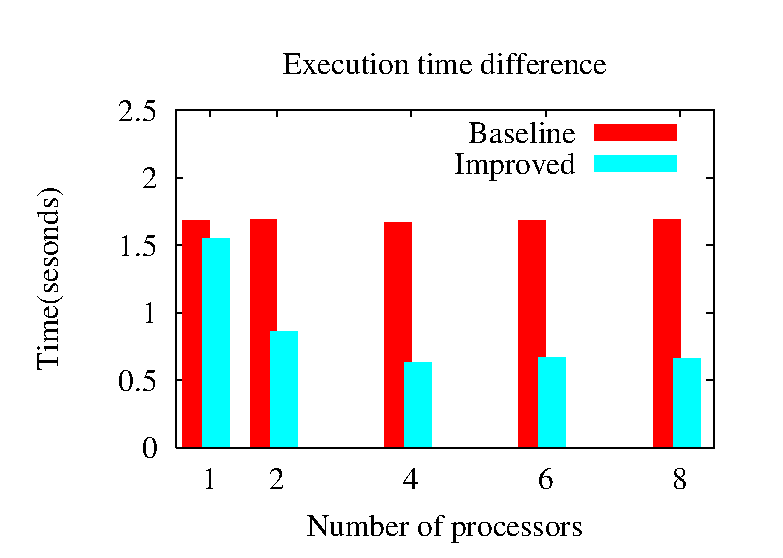
\includegraphics[angle=0, width=0.45\textwidth]{compare.eps}
%    \caption{\footnotesize Performance difference}
%    \label{fig:compare}
%  \end{center}
%\end{figure}

%Figure \ref{fig:compare} show the performance difference of the
%generated code on the POWER4 system. We set \texttt{N} as 100 and
%measured 100 times of the loop nest. In the figure, ``Baseline'' and
%``Improved'' used exactly the same compiler except Algorithm
%\ref{alg:permutepar} is not enabled in the baseline situation. We can
%see that parallel setup overhead completely offset the parallel gains
%in the first case, while the improved version get reasonable speedup
%considering such a little computation cost --- there is only one
%assign statement in the loop nest.


%\subsection{Summary of claims}
%\label{sec:claims}

%We summarize the related claims as following,

%\begin{itemize}
%\item Theorem \ref{theorem:keep}
%\item Algorithm \ref{alg:permutepar} and 
%\item its combination use with Algorithm \ref{alg:permutelocal}
%\end{itemize}

%By fine tuning the heuristics we used in Algorithm
%\ref{alg:permutepar}, we believe we can balance the need for data
%locality and coarse-grained parallelism.

\section{Summary}

Theorem \ref{theorem:keep} provides a simple way to check whether the
loop interchanged is still legal to be parallelized. We can further
use it to develop loop-permutation algorithms.

